% \documentclass[dvipdfmx, 11pt]{beamer}
\documentclass[aspectratio=169, dvipdfmx, 11pt]{beamer} % aspectratio=43, 149, 169
\usepackage{here, amsmath, latexsym, amssymb, bm, ascmac, mathtools, multicol, tcolorbox, subfig, bookmark}

% デザイン
\usetheme{Luebeck}
\usecolortheme{orchid}
\usefonttheme{professionalfonts}
\useinnertheme{circles}
\useoutertheme{infolines}
\setbeamercolor{title}{fg=structure, bg=}
\setbeamercolor{frametitle}{fg=structure, bg=}
\setbeamertemplate{itemize item}{\small\raise0.5pt\hbox{$\bullet$}}
\setbeamertemplate{itemize subitem}{\tiny\raise1.5pt\hbox{$\blacktriangleright$}}
\setbeamertemplate{itemize subsubitem}{\tiny\raise1.5pt\hbox{$\bigstar$}}

%しおりの文字化け解消
\usepackage{atbegshi}
\ifnum 42146=\euc"A4A2
\AtBeginShipoutFirst{\special{pdf:tounicode EUC-UCS2}}
\else
\AtBeginShipoutFirst{\special{pdf:tounicode 90ms-RKSJ-UCS2}}
\fi

\setbeamertemplate{navigation symbols}{}
\renewcommand{\kanjifamilydefault}{\gtdefault}
\newcommand{\red}[1]{\textcolor{red}{#1}}
\newcommand{\green}[1]{\textcolor{green!40!black}{#1}}
\newcommand{\blue}[1]{\textcolor{blue!80!black}{#1}}

\title[Day06]{機械学習の基礎}
\subtitle{Day06}
\author[Yudai Fujimoto]{Yudai Fujimoto}
\institute[SUS]{Suwa University of Science}
\date{\today}

\begin{document}
\maketitle

\begin{frame}{目次}
    \tableofcontents
\end{frame}

\section{モデルの性能の評価}
\begin{frame}{モデルの性能の評価}
    機械学習の目的は未知のデータに対して正しい予測を行うことである。\\
    そのためには、モデルを入念に評価する必要がある。ここでは以下の2つの手法を紹介する。
    \vspace{1em}
    \begin{alertblock}{ホールドアウト法(holdout method)}
        訓練データを3つのサブセットに分割して、モデルの評価を行う手法。
    \end{alertblock}
    \vspace{1em}
    \begin{exampleblock}{k分割交差検証(k-fold cross-validation)}
        訓練データセットをに\(k\)分割するして、モデルの評価を行う手法
    \end{exampleblock}
\end{frame}

\begin{frame}{ホールドアウト法}
    モデルを学習用、検証用、テスト用に分割する。
    学習には学習用データを用いて、検証用データを使用しながらハイパーパラメータを調整する。
    最終的なモデル性能の評価はテスト用のデータを使用する。
    \vspace{1em}
    \begin{figure}[b]
        \begin{center}
        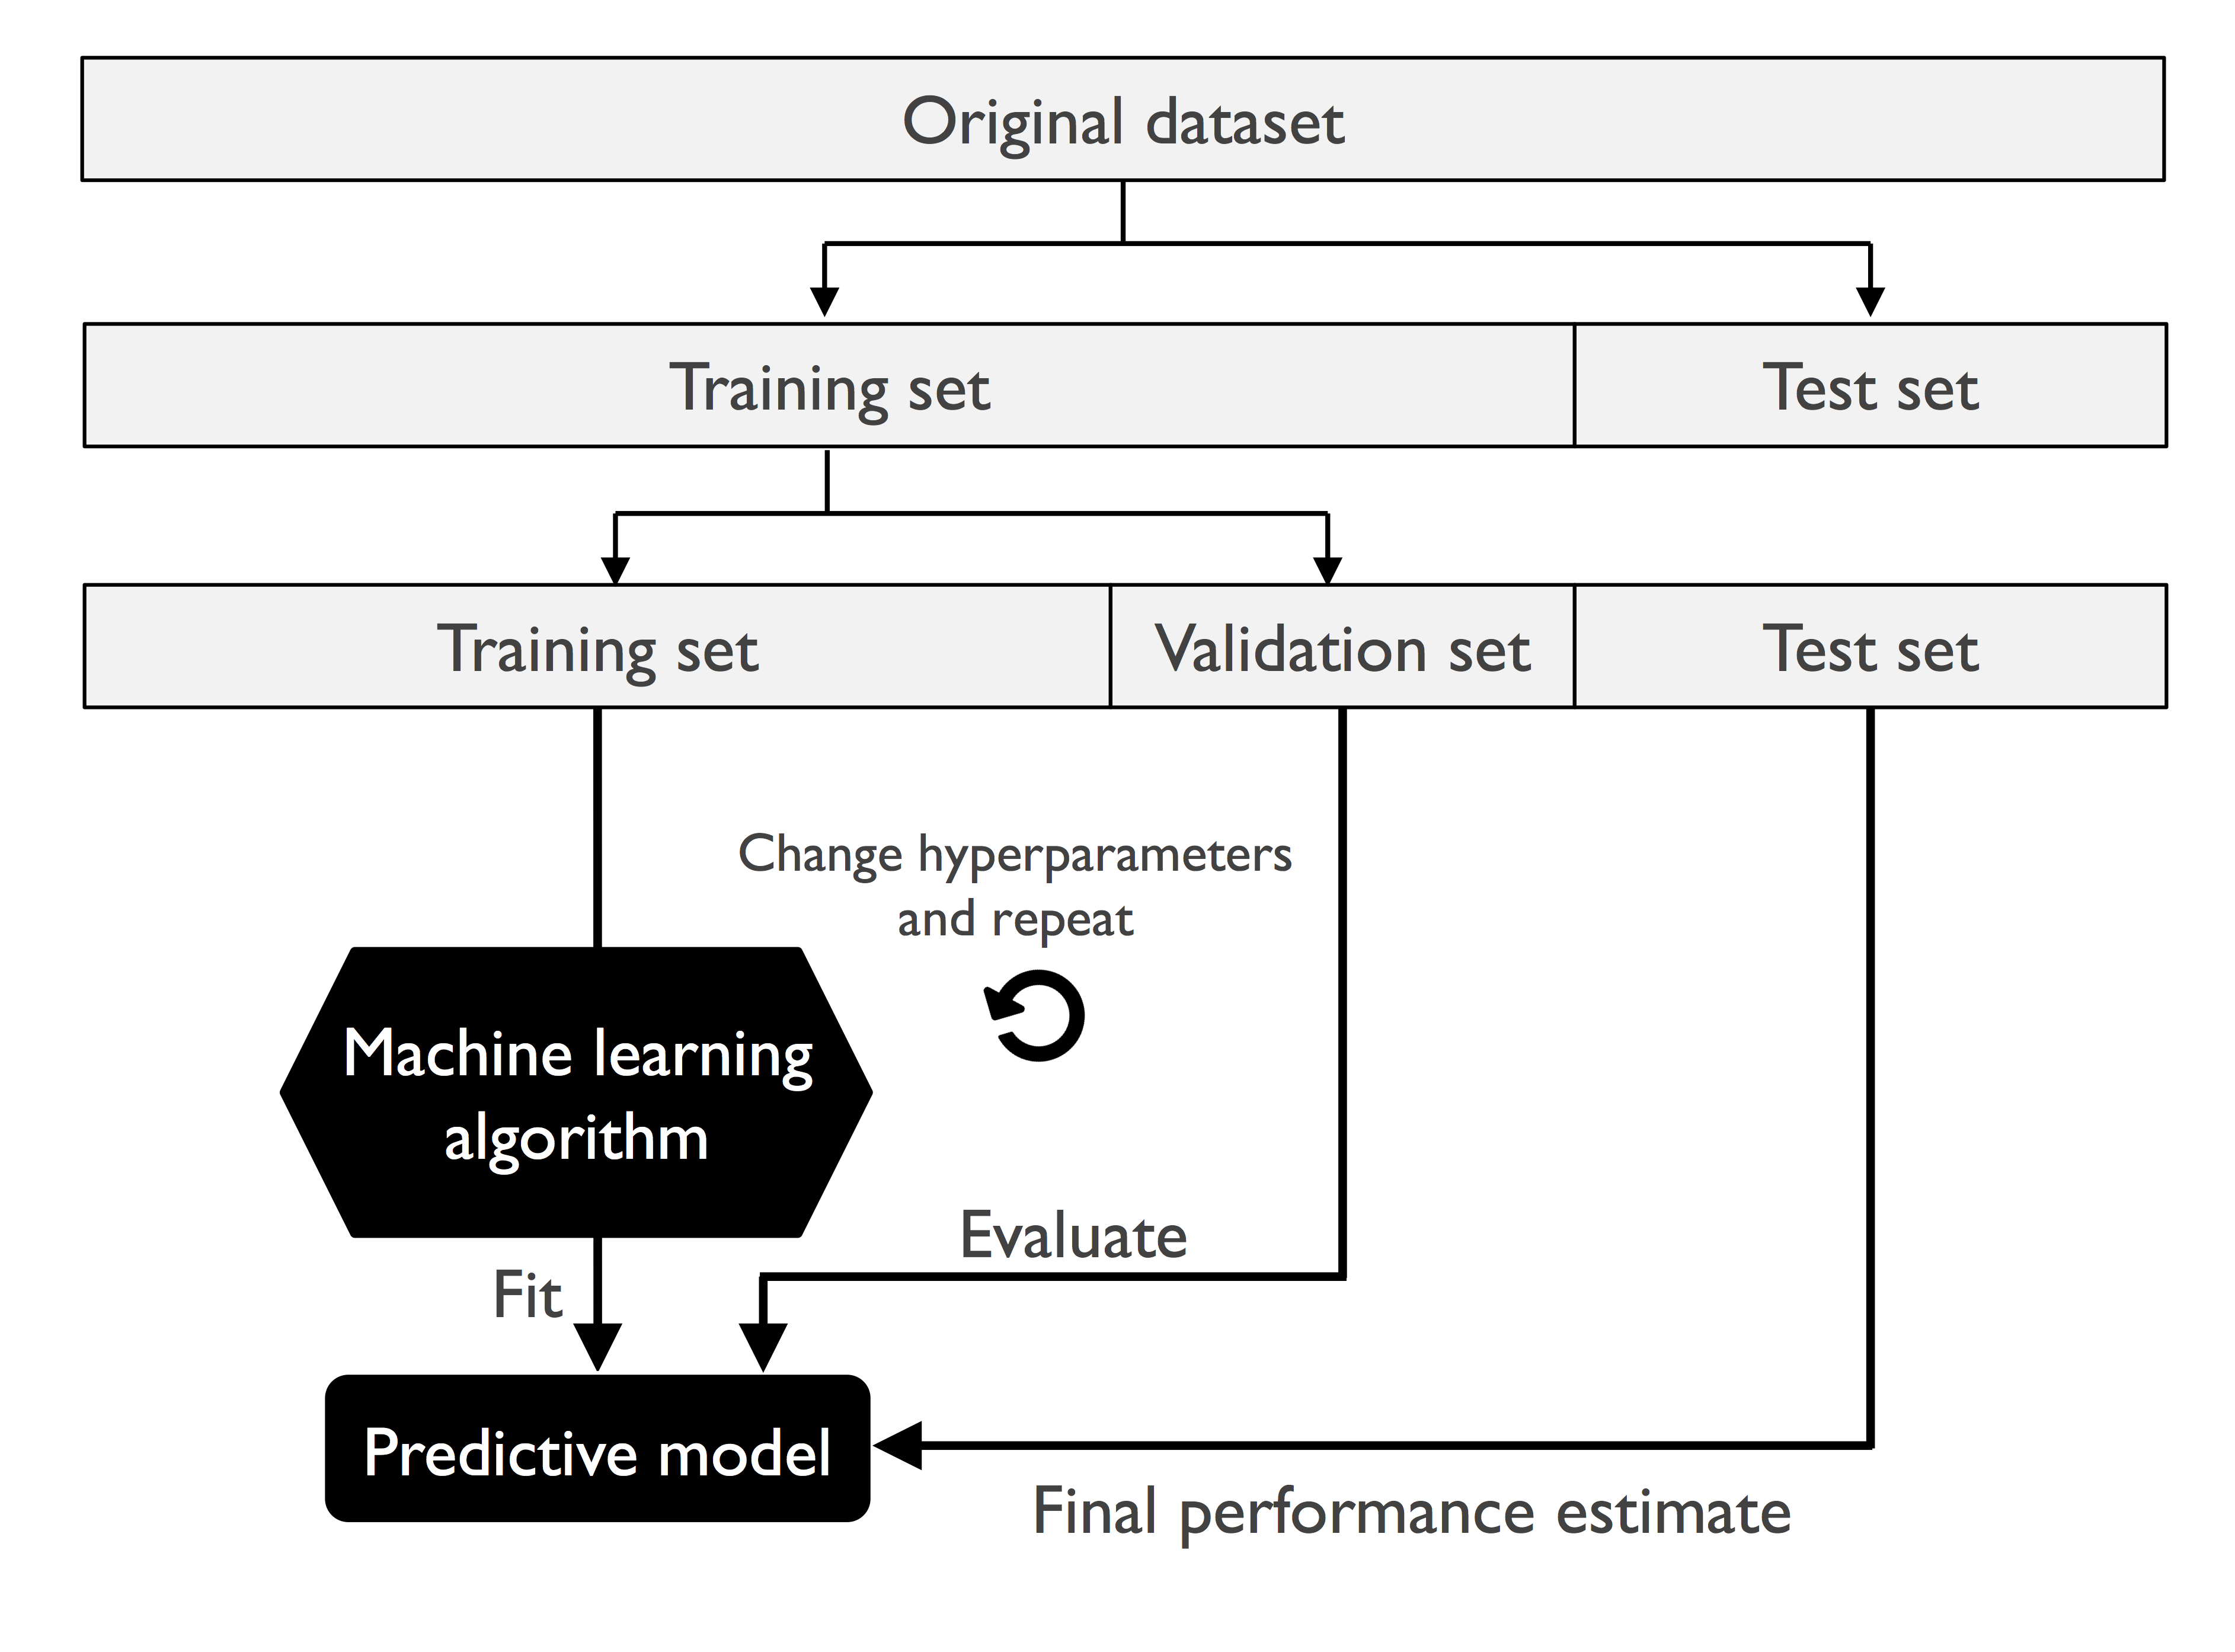
\includegraphics[width=70mm]{img/day06/fig01.png}
        \end{center}
    \end{figure}
\end{frame}

\begin{frame}{k分割交差検証}
    非復元抽出を用いて、訓練データセットをランダムに\(k\)分割する。\\
    そのうち\(k-1\)個をモデルの学習に使用し、残りの1つを性能の評価に使用する。\\
    この手順を\(k\)回繰り返すことで、\(k\)個のモデルを取得し、性能を推定する。\\
    \vspace{1em}
    \begin{figure}[b]
        \begin{center}
        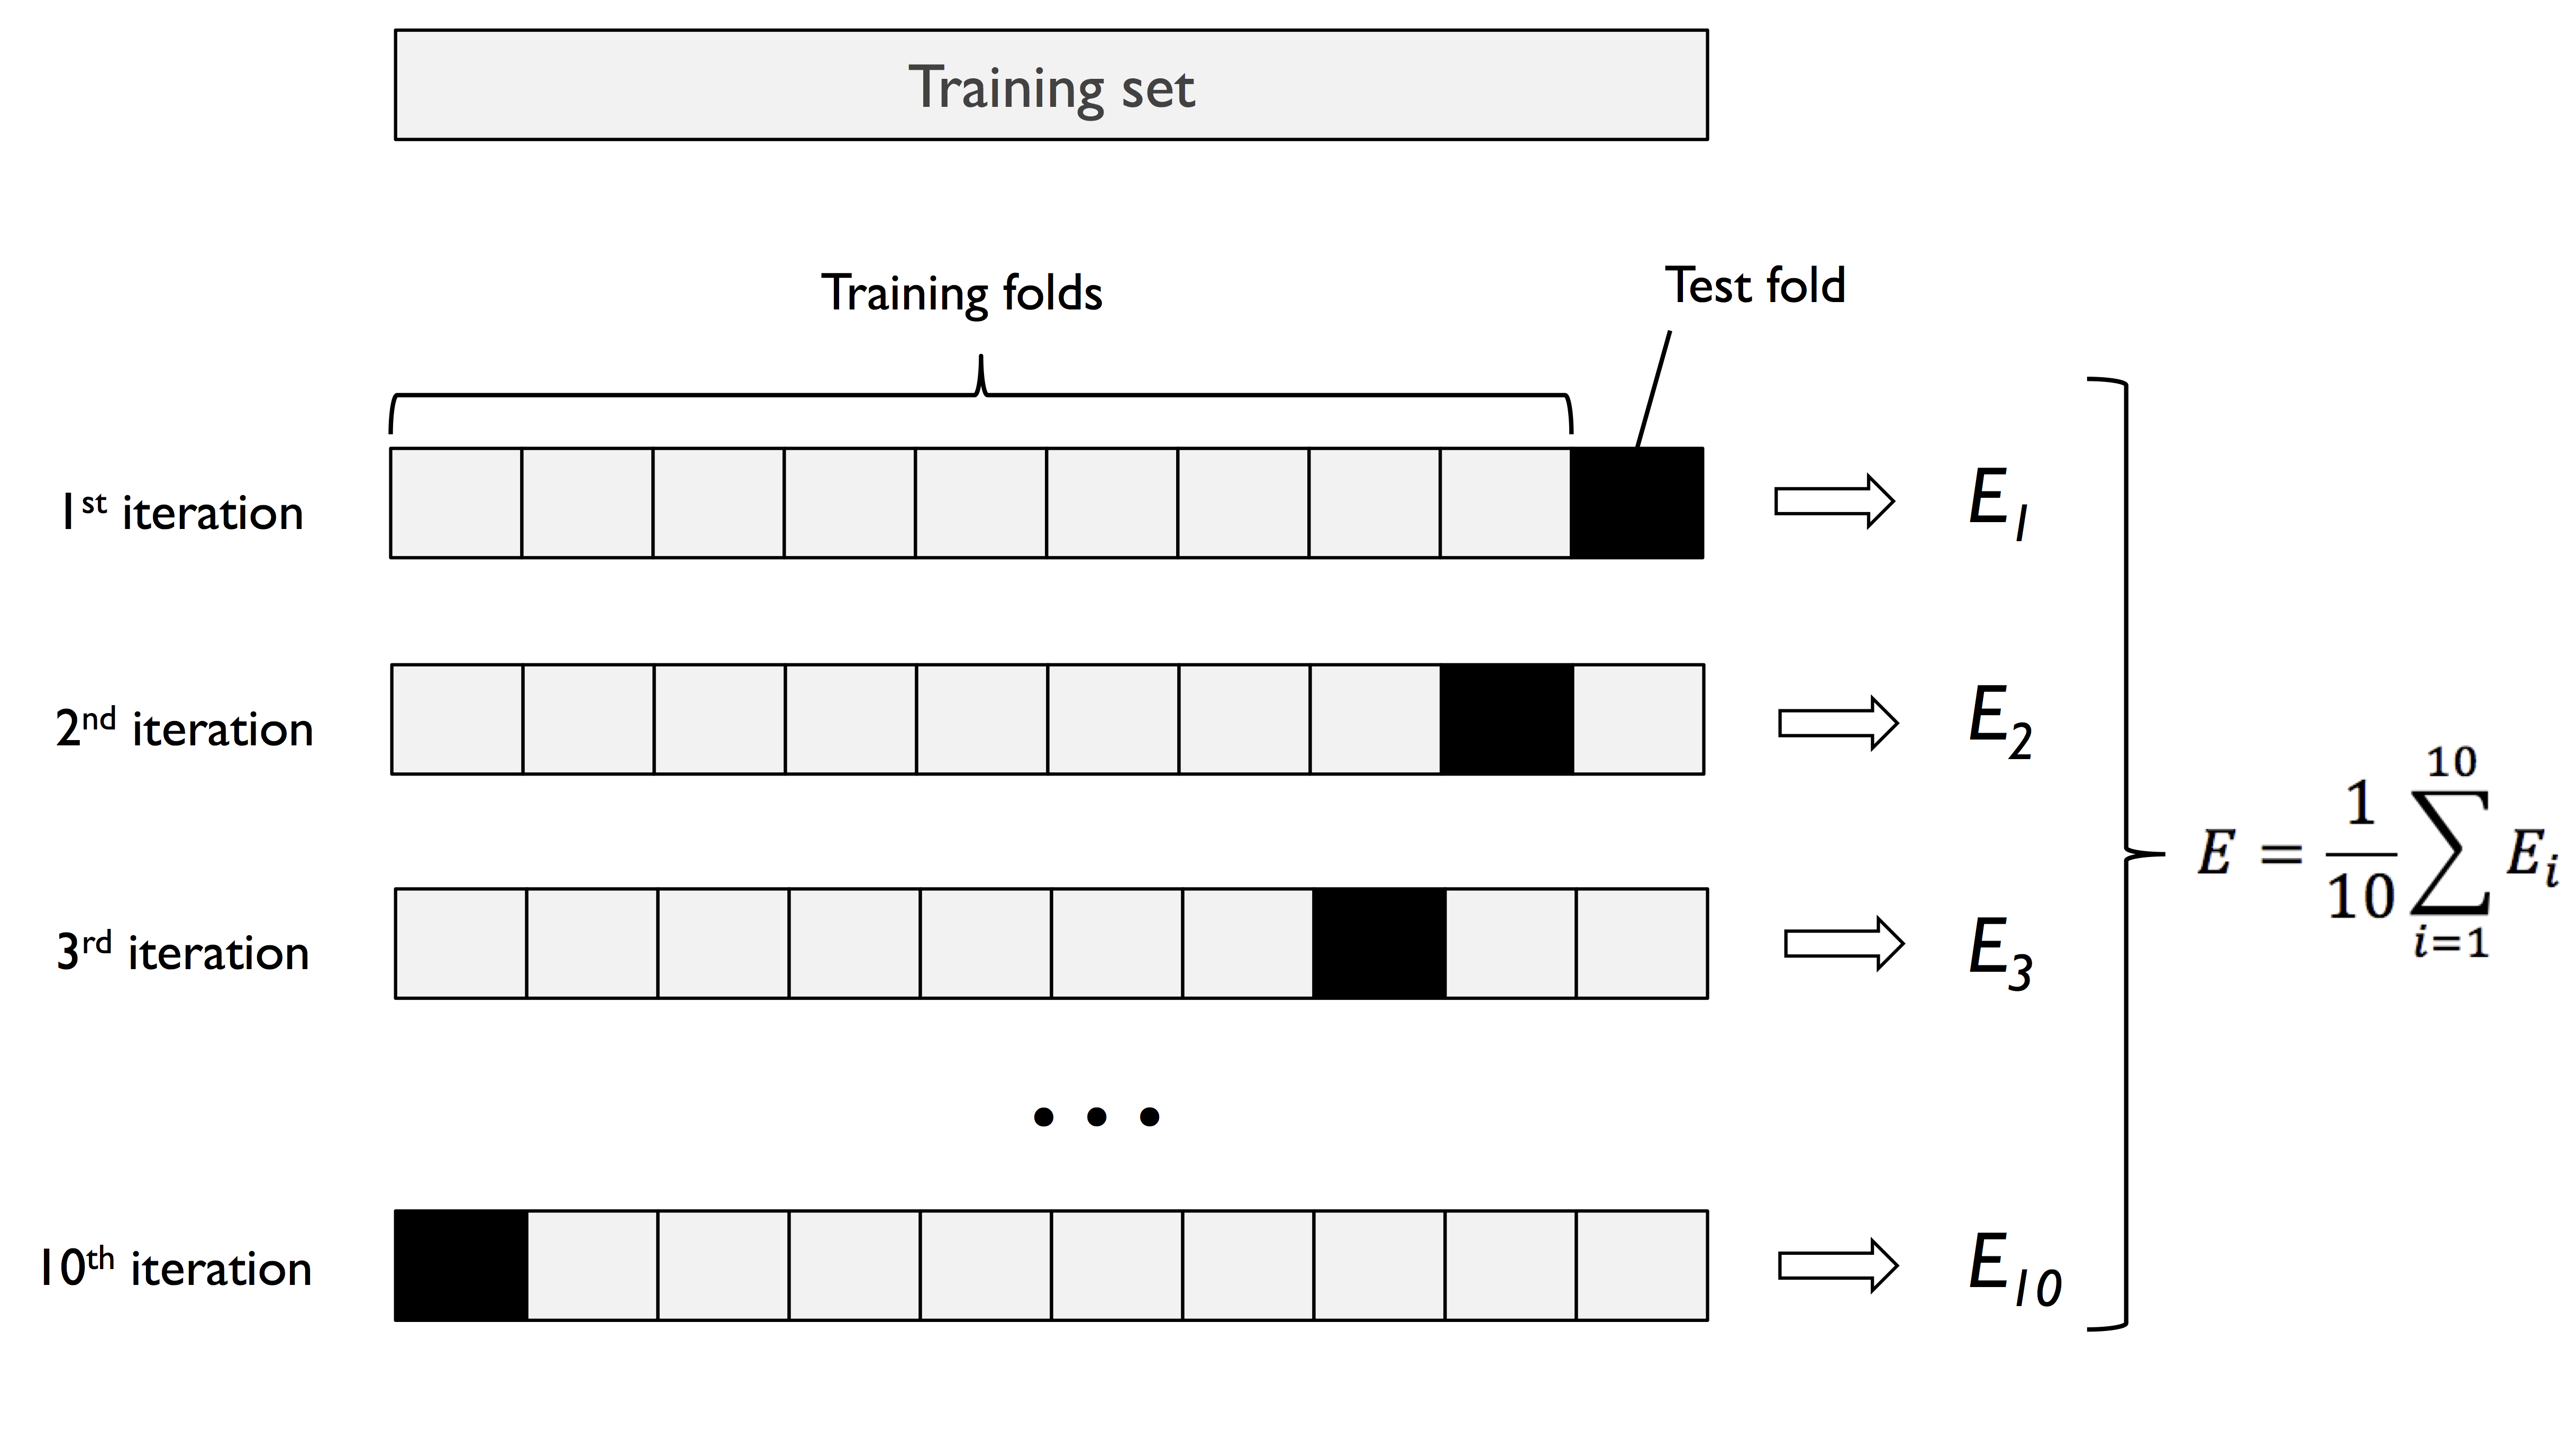
\includegraphics[width=80mm]{img/day06/fig02.png}
        \end{center}
    \end{figure}
\end{frame}

\section{アルゴリズムの診断}
\begin{frame}{アルゴリズムの診断}
    学習/検証曲線をプロットすることで、バイアスやバリアンスが高いか確認することができる
    \vspace{1em}
    \begin{figure}[b]
        \begin{center}
        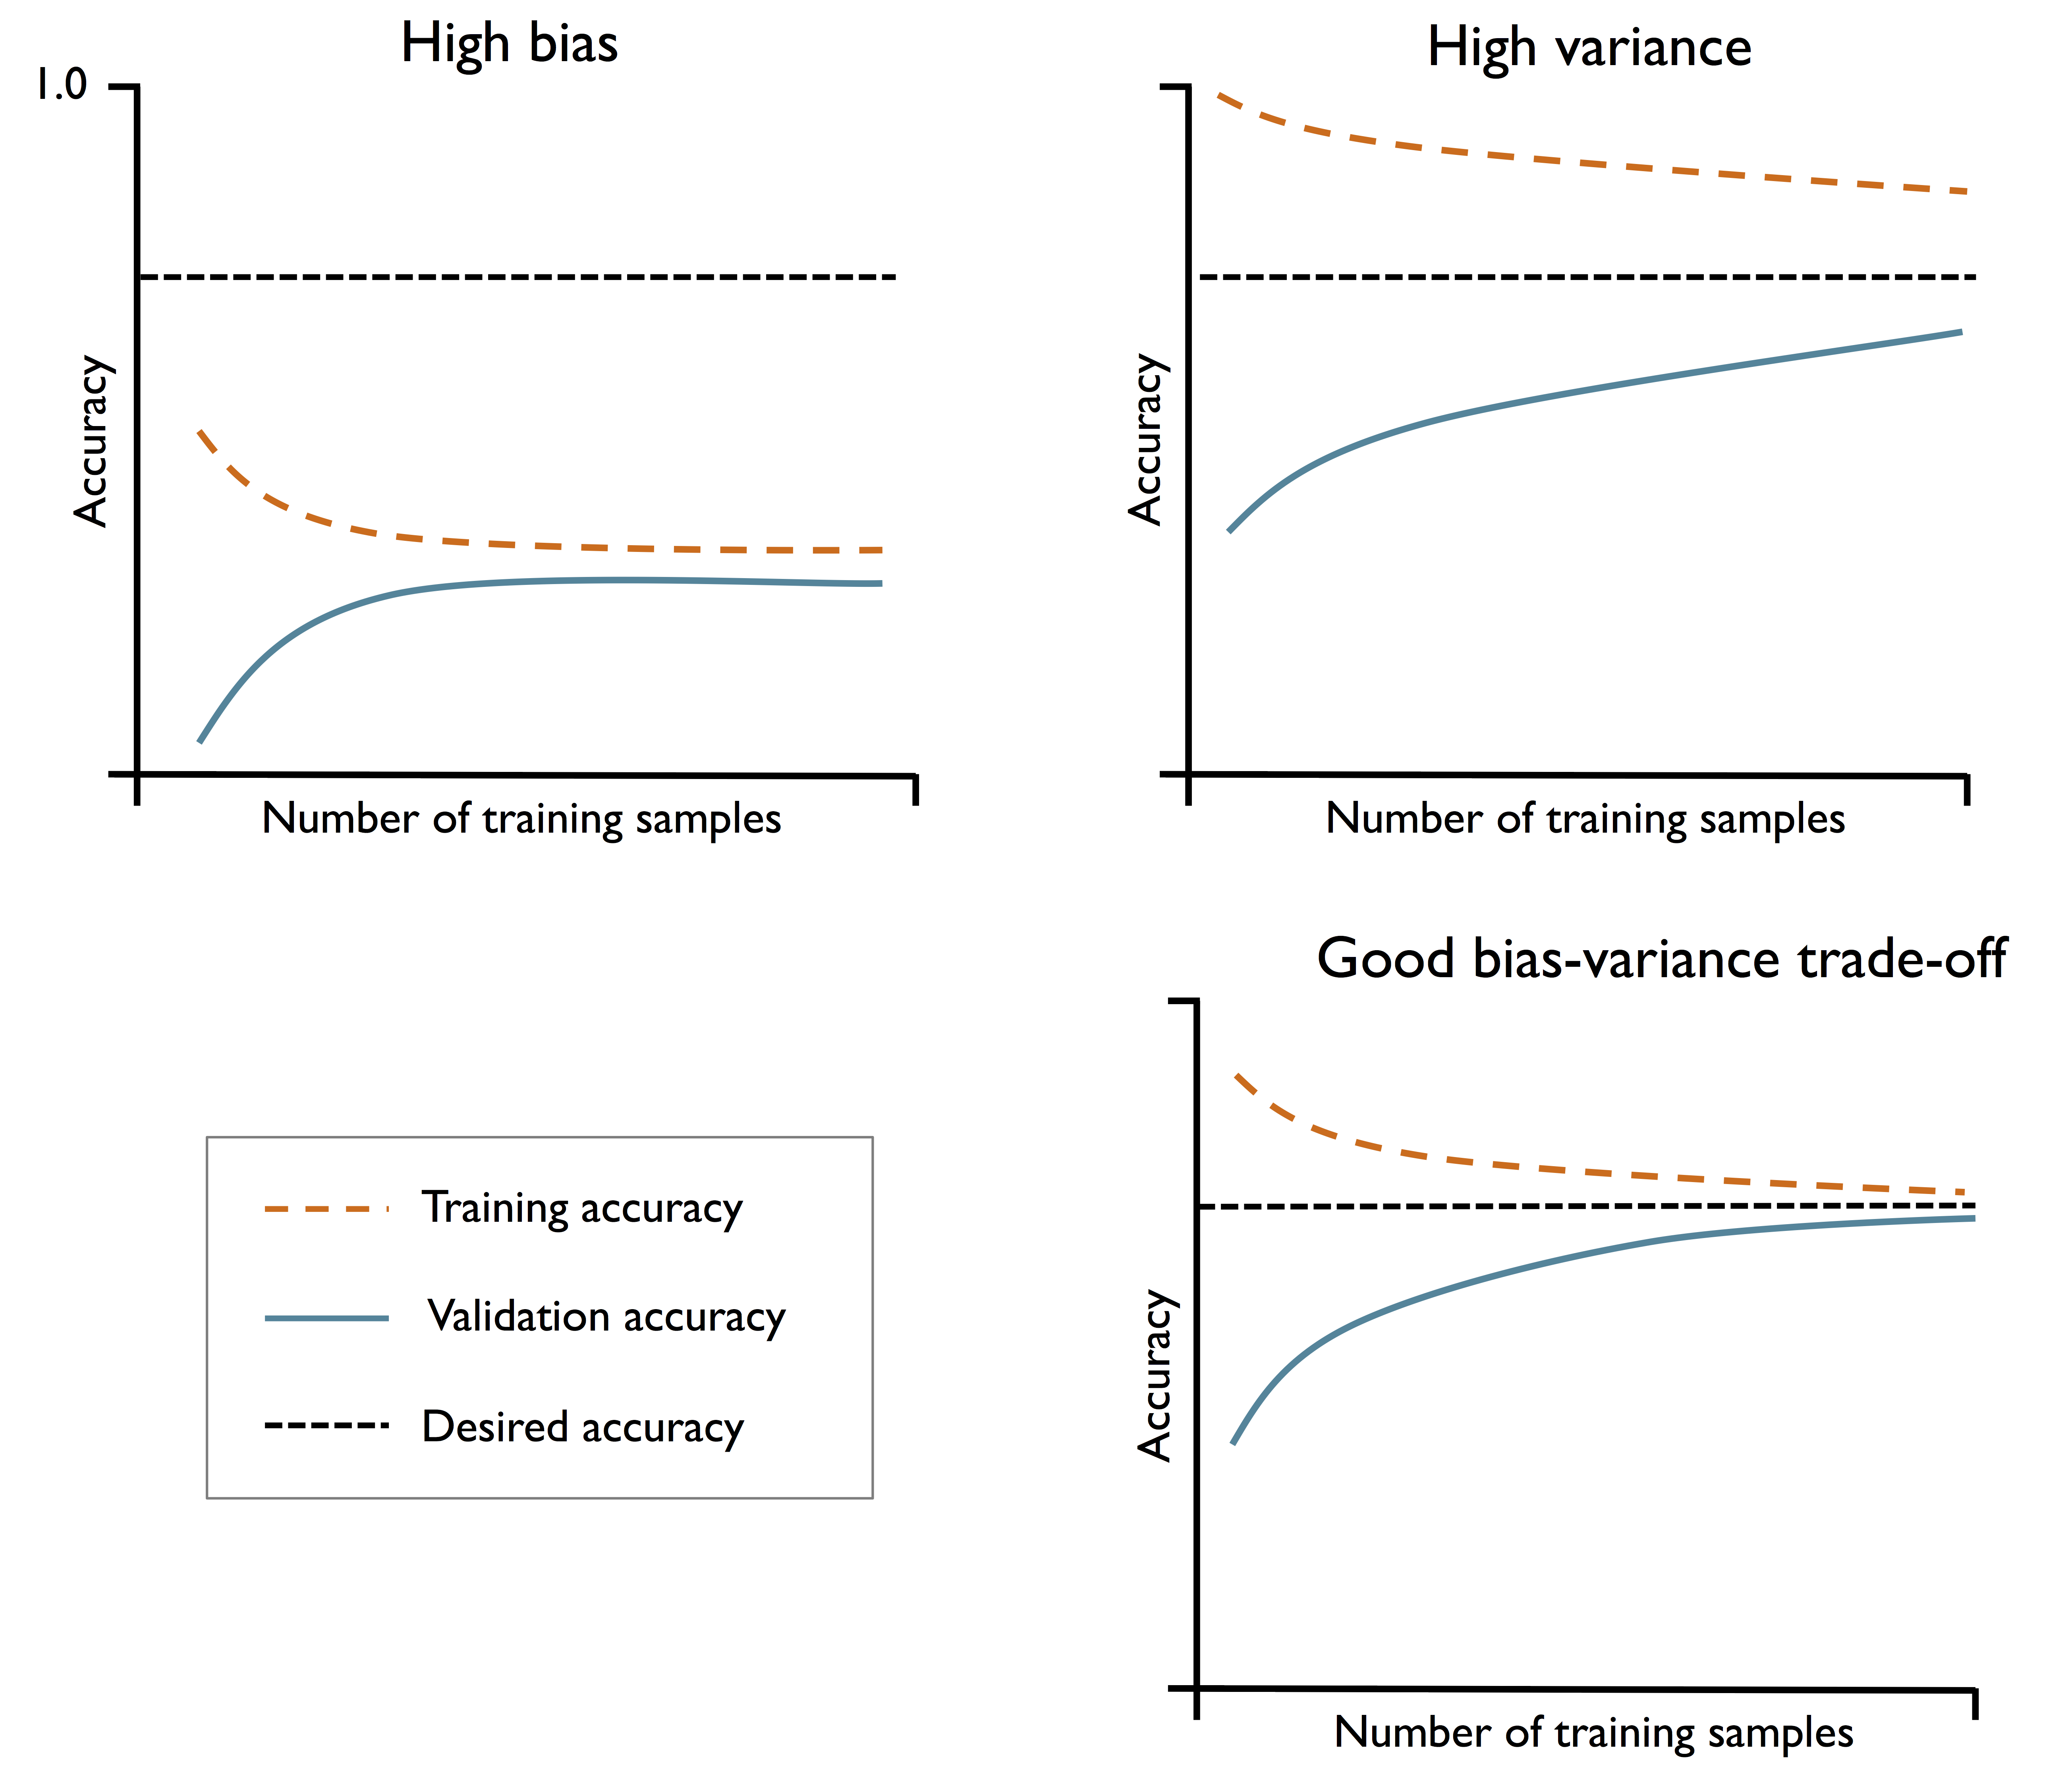
\includegraphics[width=70mm]{img/day06/fig03.png}
        \end{center}
    \end{figure}
\end{frame}

\section{パラメータチューニング}
\begin{frame}{パラメータチューニング}
    機械学習アルゴリズムにはハイパーパラメータを設定するものが多く存在する。\\
    最適なハイパーパラメータを自動で発見するには以下の手法を利用するのが良い。
    \vspace{1em}
    \begin{alertblock}{グリットサーチ}
        ハイパーパラメータの値をしらみ潰しに試して、最適な値を発見する手法、計算量はあまり良くない。
    \end{alertblock}
    \vspace{1em}
    \begin{exampleblock}{ベイズ最適化}
        ベイズ最適化を利用して効率よく、最適値を見つける。グリットサーチと比べて細かい値を発見できる。
    \end{exampleblock}
\end{frame}

% \begin{frame}{入れ子式交差検証}
%     この種の交差検証は\(5 \times 2\)交差検証と呼ばれる。
%     \vspace{1em}
%     \begin{figure}[b]
%         \begin{center}
%         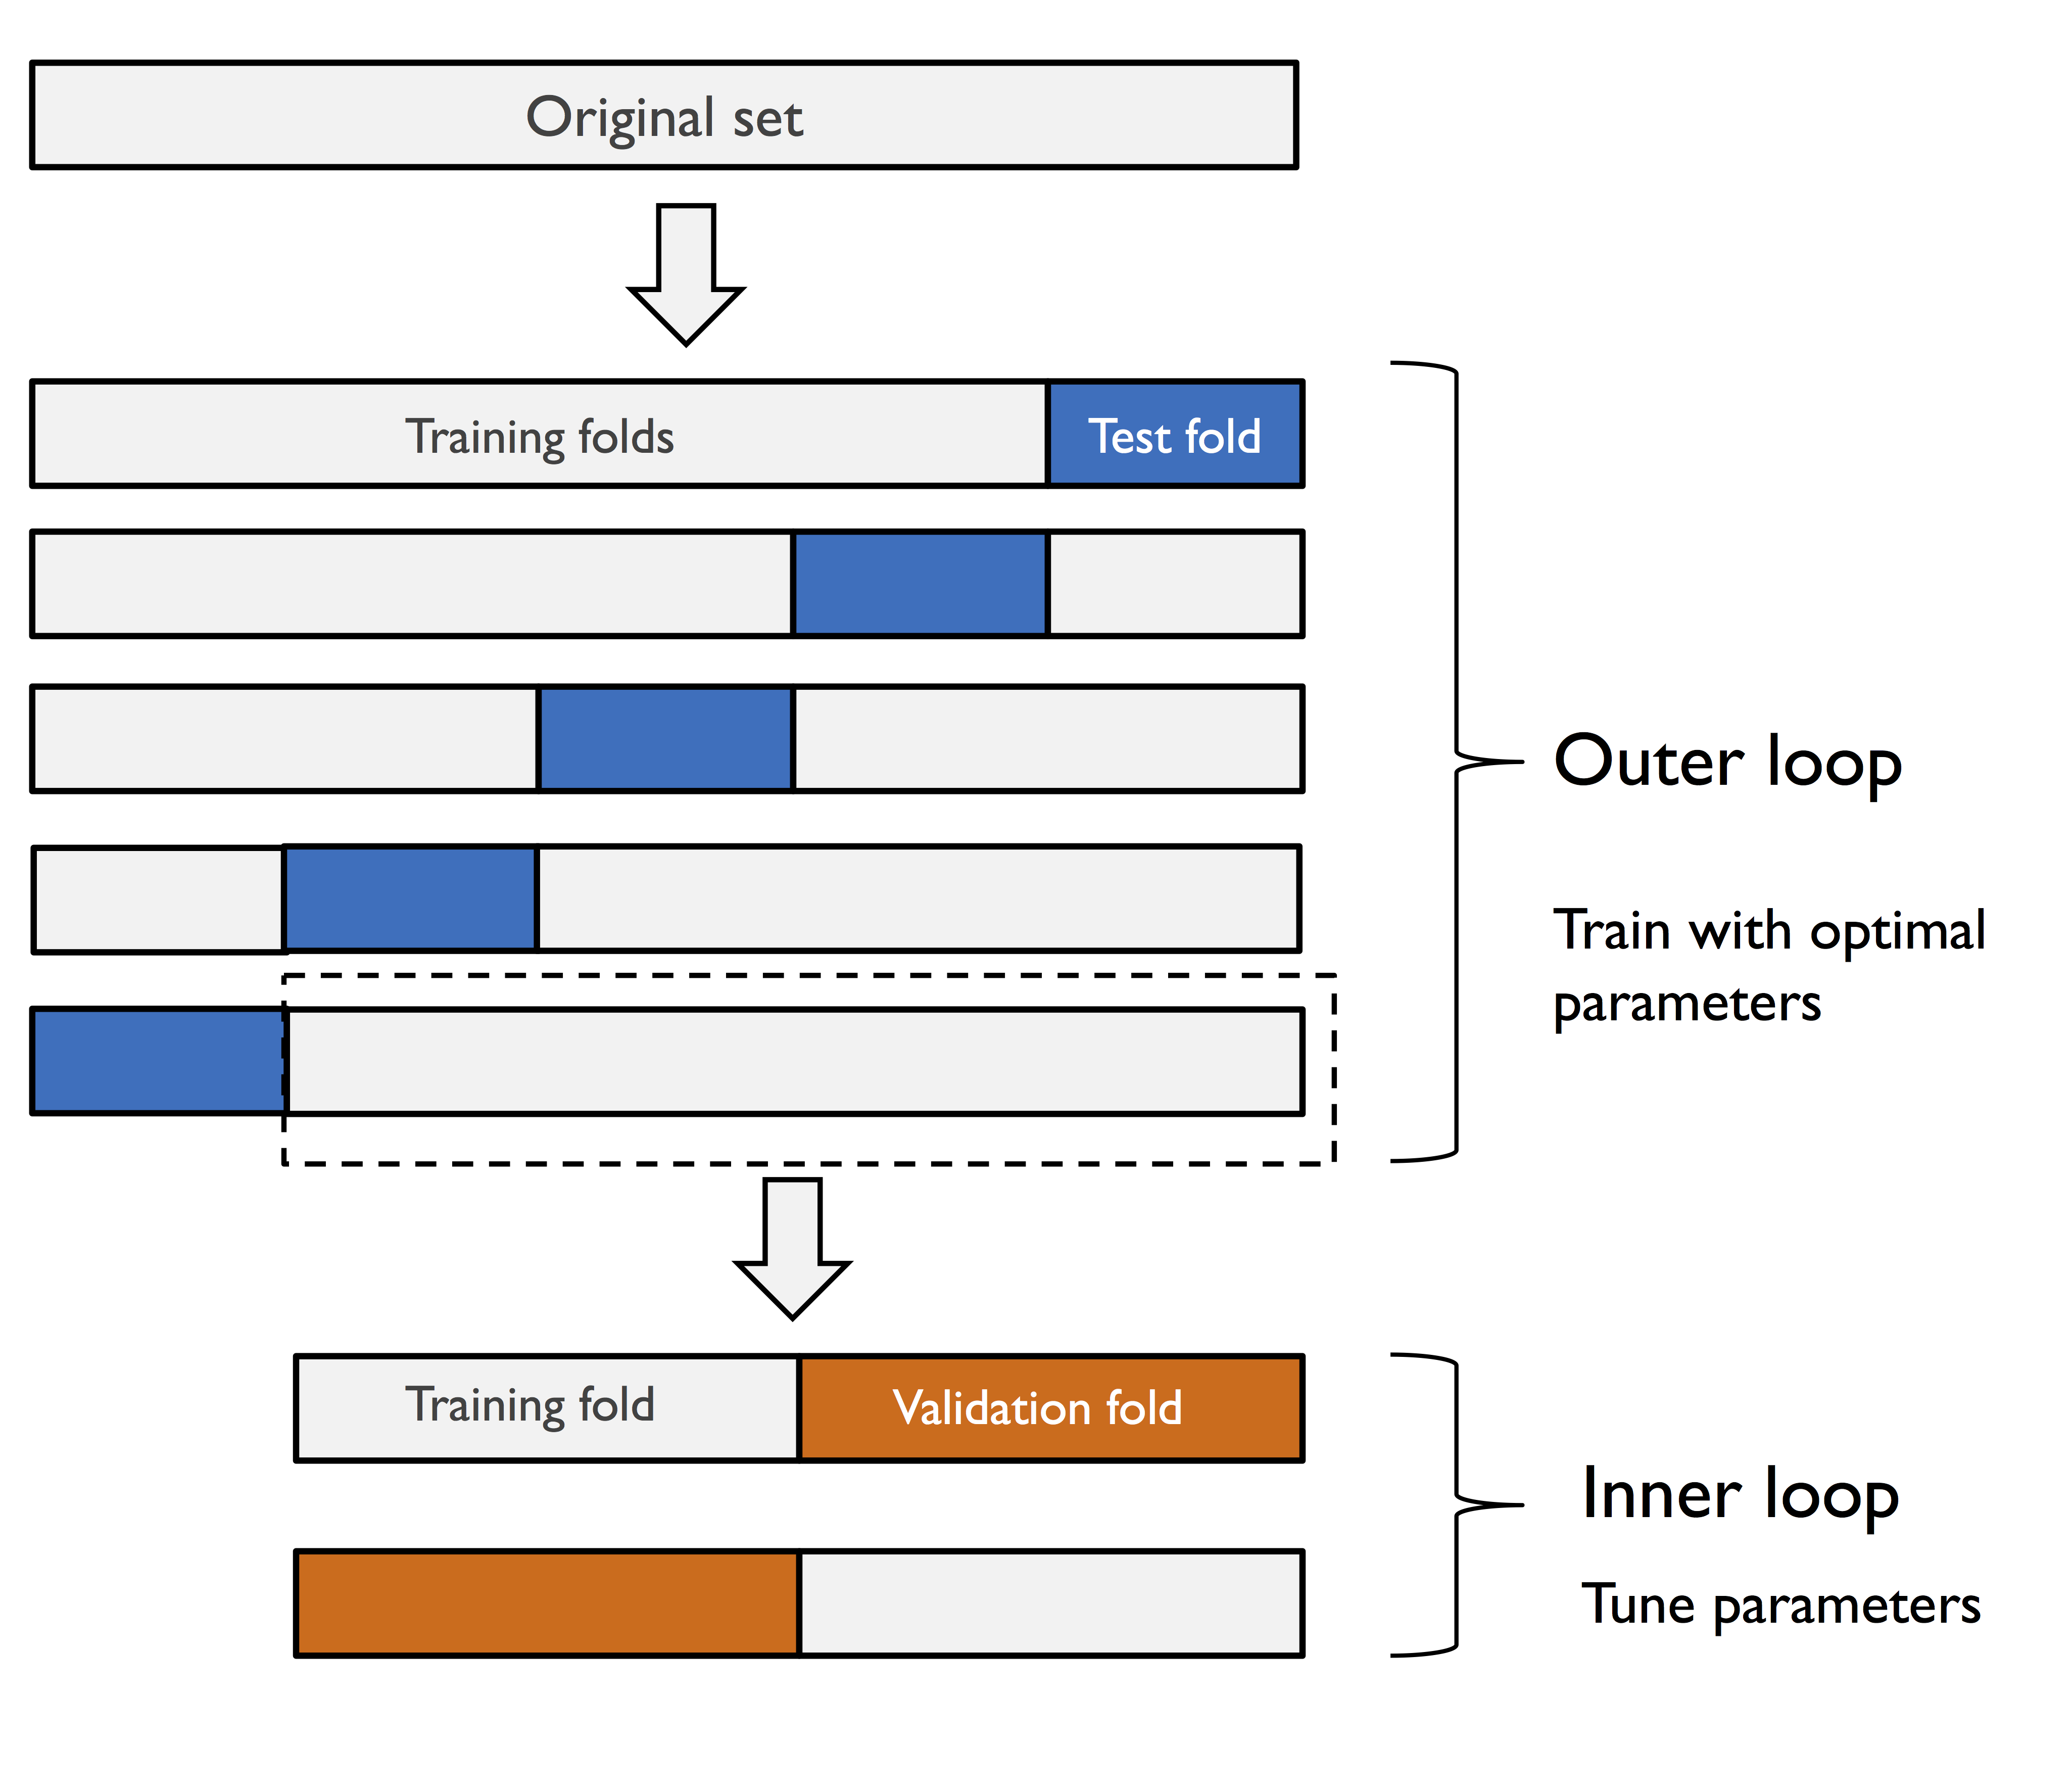
\includegraphics[width=70mm]{img/day06/fig04.png}
%         \end{center}
%     \end{figure}
% \end{frame}



\section{性能評価指標}
\begin{frame}{混合行列}
    混合行列は学習アルゴリズムの性能を明らかにする正方行列で、
    分類機の真陽性(true positive)、真陰性(true negative)、偽陽性(false positive)、
    偽陰性(false negative)からなっている。
    \vspace{1em}
    \begin{figure}[b]
        \begin{center}
        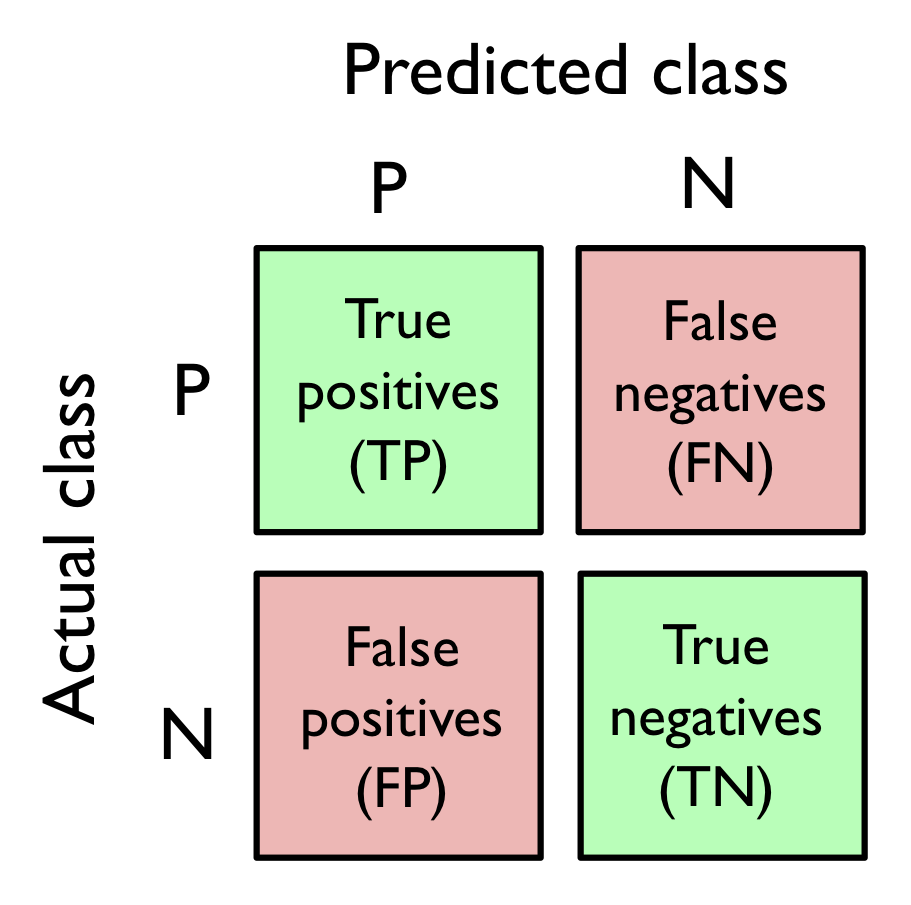
\includegraphics[width=50mm]{img/day06/fig05.png}
        \end{center}
    \end{figure}
\end{frame}

\begin{frame}{適合率と再現率}
    予測の誤分類率(ERR)と正解率(ACC)はご分類されたデータ点の個数に関する情報を示す。\\
    誤分類率は誤った予測の合計を予測の総数で割ったものと解釈できる。
    \begin{equation*}
        ERR = \frac{FP+FN}{FP+FN+TP+TN}
    \end{equation*}
    正解率は誤分類率から直接求めることができる
    \begin{equation*}
        ACC = ERR = \frac{TP+TN}{FP+FN+TP+TN} = 1 - ERR
    \end{equation*}
\end{frame}

\begin{frame}{適合率と再現率}
    真陽性率と偽陽性率は不均衡なクラスの問題で役立つ指標である。
    \begin{equation*}
        FRR = \frac{FP}{N} = \frac{FP}{FP+TN}
    \end{equation*}
    \begin{equation*}
        TRR = \frac{TP}{N} = \frac{TP}{FN+TP}
    \end{equation*}
    例として、病気の診断では、悪性の病気を検出することが重要となる。\\
    ただし、患者を不安にしないために悪性として誤分類される症状を減らすことが重要になる。
\end{frame}

\begin{frame}{ROC曲線}
    あああ
\end{frame}

\begin{frame}{他クラス分類}
    あああ
\end{frame}

\begin{frame}{クラスの不均衡}
    あああ
\end{frame}

\end{document}